\documentclass{rbfin}
\usepackage{amsmath}
\usepackage{amssymb} %mathbb
\usepackage{gensymb} % \degree
\usepackage{graphicx}
\usepackage{hyperref}
\usepackage{cancel}
\newcolumntype{C}{>{$}c<{$}}


\begin{document}
\selectlanguage{brazil}
\shorttitle{Identificação de Sistemas e Estimação de Parâmetros 2022} % appears on header every other page
\rbfe{}
\autor{Vinícius Claudino Ferraz, 2022}


\large

\begin{center}
LISTA 3
\end{center}

\normalsize

\doublespacing

\section*{Questão 1}

a) Gerei cem pontos e plotei os dados na Figura 1A.

b) Adicionei dez por cento do desvio padrão do $y$ anterior multiplicando à esquerda os randômicos gaussianos (``randn''). Plotei os dados na Figura 1B.

c) A equação de regressão, ponto a ponto, é $y_i = x^\top \theta \Leftrightarrow y_i = \theta_3 x_i^2 + \theta_2 x_i + \theta_1$.

d) Portanto, precisamos da pseudoinversa de uma \textbf{matriz de regressores} de cem linhas cujas colunas são $[1, x_i, x_i^2]$ vezes um vetor cujas cem linhas são iguais a $y_i + e_i$.

e) Os parâmetros encontrados foram $[-2.468452165780984; 0.716463937117908; 1.529449567129221]$.

f) Gerei novamente mil pontos, como em (a), e plotei os dados na Figura 2A. Adicionei o erro como em (b) e plotei os dados na Figura 2B. Com nova matriz regressora, os parâmetros encontrados foram $[-2.019564476840127;0.702513920204115;1.507382167796436]$.

Repare que com dez vezes mais pontos, os parâmetros estimados foram bem mais próximos do ideal $[-2; 0.7; 1.5]$. Isso é explicado porque a função objetivo passou a minimizar dez vezes mais realizações de erros: $J = \sum e_i^2$.

g) Gerei mais cem pontos, como em (a), e plotei os dados na Figura 3A. 

Adicionei dez por cento do desvio padrão do $x$ anterior multiplicando à esquerda os randômicos gaussianos. Plotei os dados na Figura 3B. Repare que o modo de plotagem precisa ser diferente, uma vez que o vetor $x$ tornou-se desordenado.

Com nova matriz regressora, os parâmetros encontrados foram 

$[-1.715120009257206;0.501563604178347;1.440498754963116]$.

Repare que o resultado foi o menos preciso.

A comparação dos $(x_2,y_2),(x_3,y_3),(x_4,y_4)$ montados após a regressão foi plotada na Figura 4. Repare que a diferença entre as aproximações é mínima diante do total dos dados.

\begin{center}
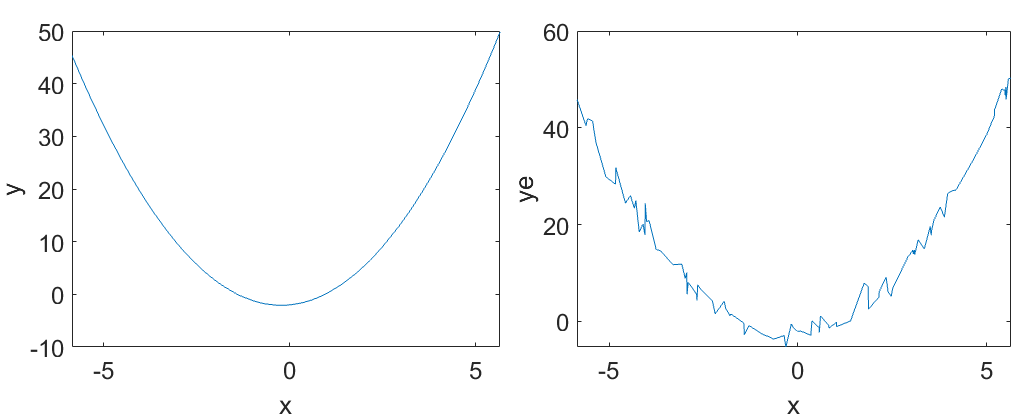
\includegraphics[scale=0.65]{1 gera 100}
Figura 1: 100 pontos gerados (a) sem erro (b) com erro na saída.
\end{center}

\begin{center}
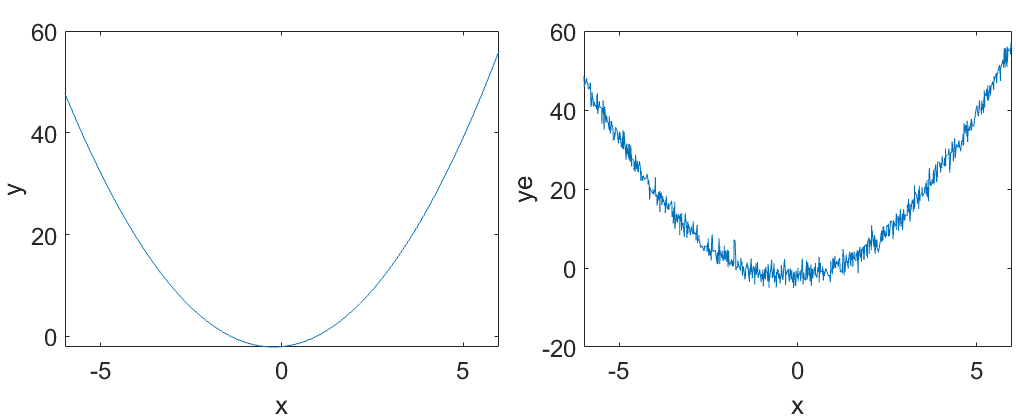
\includegraphics[scale=0.65]{2 gera 1000}
Figura 2: 1000 pontos gerados (a) sem erro (b) com erro na saída.
\end{center}

\begin{center}
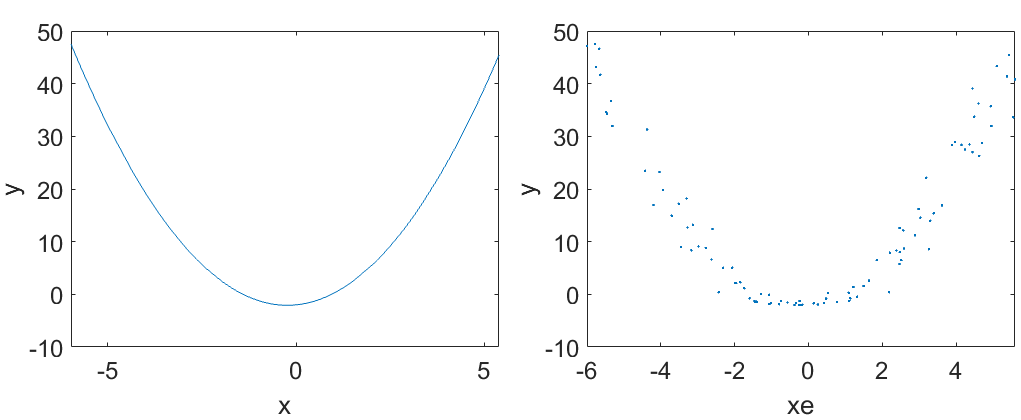
\includegraphics[scale=0.65]{3 gera mais 100}
Figura 3: 100 pontos gerados (a) sem erro (b) com erro na entrada.
\end{center}

\begin{center}
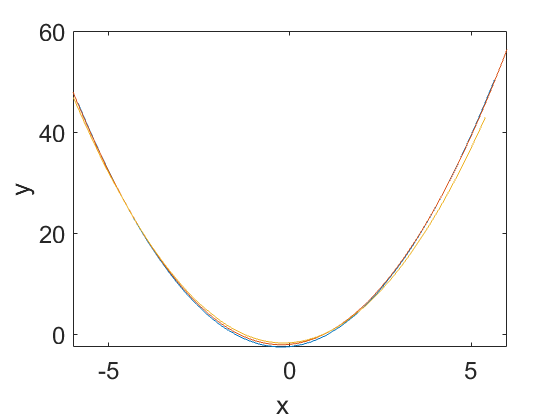
\includegraphics[scale=0.666]{4 regredidos}

Figura 4: comparação utilizando os 3 vetores $\theta$ de parâmetros encontrados.
\end{center}

\section*{Questão 2}

a) A entrada é $prbs(n,12,1)$, subtraída a média, multiplicada por $2$, plotada na Figura 5A.

O ruído $\nu$ (plotado na Figura 5B) são os gaussianos ``randn'' multiplicados por $\sqrt{0.1}$. Vou explicar essa constante.

Pela definição de variância, se nós tivermos $var(X) = E[X^2] - E^2[X] = v$

$\Rightarrow E[X^2] = v + c^2$, então ao multiplicarmos por uma constante $k$, 

$var(kX) = E[k^2 X^2] - E^2[kX] = w \Rightarrow k^2 \underbrace{E[X^2]}_{v + c^2} - (ck)^2 = w$.

$\therefore k = \pm \sqrt{\cfrac{w}{v}}$ é a constante desejada.

b) Modelo ARX (plotado na Figura 6A):

$Ay = Bu + \nu$

$y(k) = - \theta(1) y(k-1) - \theta(2) y(k-2) + \theta(3) u(k - 1) + \theta(4) u(k - 2) + \nu(k)$.

c) Modelo ARMAX (plotado na Figura 6B):

$Ay = Bu + C \nu$ ; Repare que troquei $A, B, C$ por $\theta$, para futura estimação.

$y(k) = - \theta(1) y(k-1) - \theta(2) y(k-2) + \theta(3) u(k - 1) + \theta(4) u(k - 2) + \theta(5) \nu(k) + \theta(6) \nu(k - 1)$.

d) Modelo com erro na saída (plotado na Figura 7):

$Fw = Bu$ ; $y = w + \nu$ ; Repare que é o único sem filtro. Não há função de $q$ multiplicando $\nu$.

$w(k) = - \theta(1) w(k-1) - \theta(2) w(k-2) + \theta(3) u(k - 1) + \theta(4) u(k - 2)$ ; $y(k) = w(k) + \nu(k)$.

\begin{center}
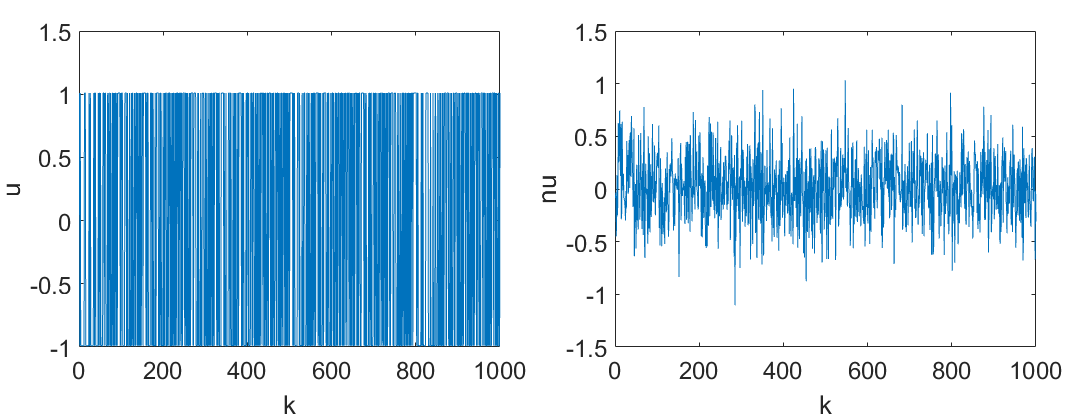
\includegraphics[scale=0.65]{5a}
Figura 5: (a) entrada (b) ruído.
\end{center}

\begin{center}
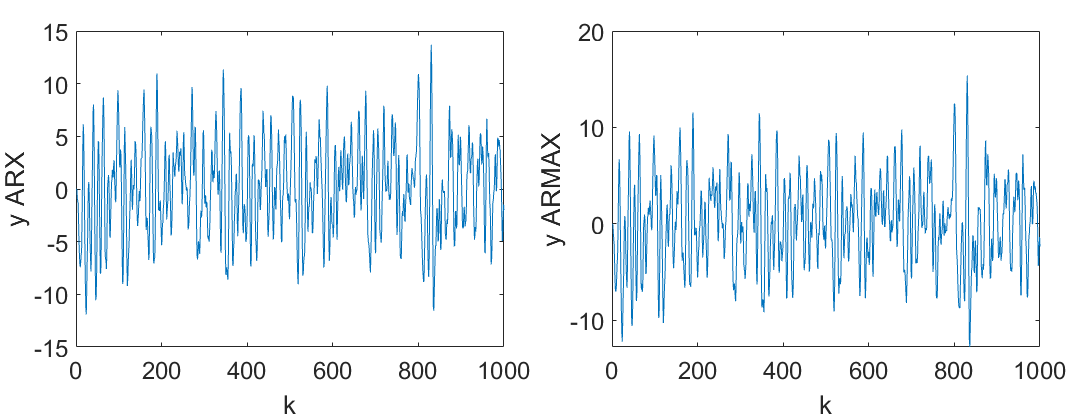
\includegraphics[scale=0.65]{6a}
Figura 6: Simulações: (a) ARX (b) ARMAX.
\end{center}

\newpage

\begin{center}
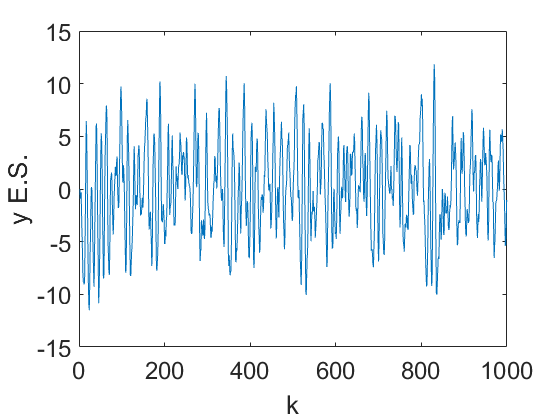
\includegraphics[scale=0.666]{7}

Figura 7: Simulação com erro na saída.
\end{center}


\section*{Questão 3}

Os parâmetros ideais são $[-1.5; 0.7; 1; 0.5; 1; 0.8]$. Veremos que não é possível estimar os dois últimos.

a) ARX: Temos $y_{(3:1000)} = X \theta$, em que cada uma das $998$ linhas de $X$ é 

$[-y(k-1), -y(k-2), u(k - 1), u(k - 2)]$. Os parâmetros encontrados foram: 

$[-1.492231811181352;0.691822104421257;0.991675629125383;0.498357708396526]$.

Foi possível montar toda a matriz de regressão.

b) ARMAX: Não foi possível montar toda a matriz de regressão. Para isso, teríamos que ter disponíveis os dados de $\nu$. Os parâmetros encontrados foram: 

$[-1.511287691284849;0.709024279287422;1.001511280557228;0.472411376814075]$.

c) Erro na saída: os parâmetros encontrados foram: 

$[-1.428278426942452;0.632047338684911;0.973519519942481;0.582697779355300]$.

O que acontece aqui é que nós precisaríamos de colunas com os valores de $w = y - \nu$ que foram trocadas por $y$. Portanto, foi possível estimar todos os parâmetros.

d) Sobre o desempenho. Calculando o valor da função objetivo $J = \sum e_i^2$, obtivemos 

$J_{ARX} = 96.8369$ ; $J_{ARMAX} = 155.9078$ ; $J_{ES} = 348.7046$. Dessa forma, concluímos que a aproximação mais precisa é do $ARX$, e a menos precisa é a do modelo de erro na saída.

\section*{Questão 4}

Por definição, $J_{reg} = 0.5 J_{MQ} + 0.5 \lambda \theta^\top \theta$, em que $\lambda \in \mathbb{R}$ é um escalar e $\theta \in \mathbb{R}^n$ é um vetor, a nossa incógnita a ser estimada, minimizando $J_{reg}$.

Sejam $\Psi \in \mathcal{M}_{N \times n}(\mathbb{R})$ ; $N \ge n$. Aproximamos a saída pelos parâmetros pré multiplicados pela matriz de regressão, cuja diferença é o erro $\xi \in \mathbb{R}^n$. 

$y = \Psi \hat\theta + \xi$.

Por definição, $J_{MQ} = \sum_{i = 1}^N \xi(i)^2$.

Então, $J_{MQ} = \xi^\top \xi = (y - \Psi \hat\theta)^\top (y - \Psi \hat\theta) = y^\top y - y^\top \Psi \hat\theta - \hat\theta^\top \Psi^\top y +  \hat\theta^\top \Psi^\top \Psi \hat\theta$.

Derivando, temos que $\cfrac{\partial J_{reg}}{\partial \hat \theta} = 0.5( - \Psi^\top y - \Psi^\top y + 2 \Psi^\top \Psi \hat \theta + 2 \lambda \hat \theta)$

O mínimo acontece quando a derivada é zero:

$\cfrac{\partial J_{reg}}{\partial \hat \theta} = 0\Rightarrow - \Psi^\top y + \Psi^\top \Psi \hat \theta + \lambda \hat \theta = 0 \Rightarrow (\Psi^\top \Psi + \lambda I) \hat \theta = \Psi^\top y$.

Finalmente, pré-multiplicando pela inversa dos dois lados:

$\hat \theta_{reg} = [\Psi^\top \Psi + \lambda I]^{-1} \Psi^\top y$.

O que fizemos foi minimizar $J_{reg} = \sum_{i = 1}^N \xi(i)^2 + \sum_{i = 1}^n \theta(i)^2 = \Vert \xi \Vert^2 + \Vert \theta \Vert^2$. Essa constante $0.5$ é desprezível nesse caso. Portanto, a norma dos parâmetros também será mínima.

\vspace{6mm}

Link para os \href{https://drive.google.com/file/d/1iwa1n0PrfYBjP0JjEgHDD2WnVX3Xsz3W/view?usp=sharing}{\color{blue}\underline{códigos-fonte}}.

Versão de 13/maio/2022\footnote{Fora da caridade não há salvação.} por Vinicius Claudino Ferraz. 

Matrícula: 2019435823.

\end{document}
